\documentclass[12pt, twoside]{report}
\usepackage[utf8]{inputenc}
\usepackage[croatian]{babel}
\usepackage{graphicx}
\graphicspath{ {Images/} }
\usepackage{lipsum}
\usepackage[a4paper,width=150mm,top=25mm,bottom=25mm,bindingoffset=6mm]{geometry}
\usepackage{fancyhdr}
\usepackage{xcolor}
\usepackage{tcolorbox}
\usepackage{draftwatermark}
\pagestyle{fancy}
\fancyhead{}
\fancyhead[RO,LE]{Proporcionalna navigacija i upravljanje kretanja projektila}
\setlength{\headheight}{15pt}
\fancyfoot{}
\fancyfoot[CO,RE]{\thepage}
\renewcommand{\headrulewidth}{0.4pt}
\renewcommand{\footrulewidth}{0.4pt}

\SetWatermarkText{Nedovršeno}
\SetWatermarkScale{5}
% https://en.wikibooks.org/wiki/LaTeX/Floats,_Figures_and_Captions
\usepackage{caption}
\usepackage{subcaption}

% References
\usepackage[style=authoryear,sorting=ynt]{biblatex}
\addbibresource{references.bib}

% https://en.wikibooks.org/wiki/LaTeX/Text_Formatting#Line_Spacing
\usepackage{setspace}
\singlespacing
%\onehalfspacing
%\doublespacing
%\setstretch{1.1}

\begin{document}

\begin{titlepage}
    \begin{center}
        \vspace*{1cm}
        
        \Huge
        \textbf{Navigacija i upravljanje projektila}
        
        %\vspace{0.5cm}
        
       % \LARGE
        %Thesis Subtitle
        
        \vspace{1.5cm}
        
        \Large
        \textbf{Mirza Hodžic}\\
        
        \vspace{0.5cm}
        
        Mentor: prof. dr. Naser Prljača\\
        
        \vfill
        
        
\includegraphics[width=0.5\textwidth]{Images/preuzmi.png}
        
        \vspace{0.8cm}
        
        \Large
        A thesis presented for the degree of Doctor of Philosophy
        
        \vspace{0.5cm}
        
        \LARGE
	    \textsc{Fakultet eleketrotehnike\\
	    Univerzitet u Tuzli}
	    
	    \begin{flushright}
	
	    \Large
	    Date
	
	    \end{flushright}
        
    \end{center}
\end{titlepage}

%\chapter*{Dedication}
%To mum and dad...

%\chapter*{Declaration}
%I declare that..

%\chapter*{Acknowledgements}
%I want to thank...

\tableofcontents

\listoffigures

\listoftables

%\thispagestyle{plain}
\begin{center}
    \Large
    \textbf{Thesis Title}
    
    \vspace{0.4cm}
    \large
    Thesis Subtitle
    
    \vspace{0.4cm}
    \textbf{Author Name}
    
    \vspace{0.9cm}
    \textbf{Abstract}
\end{center}

\lipsum[1-3]

\chapter{Uvod}
\input{Chapters/introduction}

\chapter{Uvod u proporcionalnu navigaciju}
\section{Opis planarnog susreta}
\begin{figure}[!ht]
    \centering
    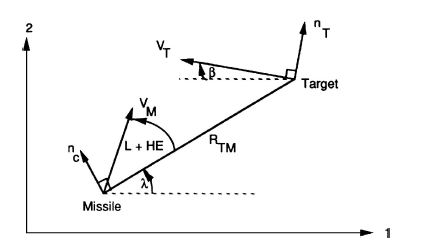
\includegraphics{PNfigure.JPG}
\end{figure}
\noindent Udaljenost između mete i projektila u svakom trenutku je data sa:
\begin{equation}
    r(t)=r_T(t)-r_M(t)
\end{equation}
Brzina približavanja projektila meti je data sa: 
\begin{equation}
    v_{cl}=-\dot{r}(t)
\end{equation}
Ugaono ubrzanje mete je dato sa:
\begin{equation}
    \dot{\beta}=\frac{n_T}{v_T}
\end{equation}
Kompnente vektora brzine mete u koordinatnom sistemu vezanom za zemlju su date sa:
\begin{equation}
    v_{T1}=-v_T\cos{\beta}
\end{equation}
\begin{equation}
    v_{T2}=v_T\sin{\beta}
\end{equation}
Slično tome, brzina i ubrzanje projektila su date sa:
\begin{equation}
    \dot{v}_{M1}=a_{M1}
\end{equation}
\begin{equation}
    \dot{v}_{M2}=a_{M2}
\end{equation}
\begin{equation}
    \dot{R}_{M1}=v_{M1}
\end{equation}
\begin{equation}
    \dot{R}_{M2}=v_{M2}
\end{equation}
Ugao \textit{Line of sight} se može izračunati kao:
\begin{equation}
    \lambda = \arctan{\frac{R_{TM2}}{R_{TM1}}}
\end{equation}
Pa je: 
\begin{equation}
    \dot{\lambda}=\frac{R_{TM1}v_{TM2}-R_{TM2}v_{TM1}}{r^2}
\end{equation}
Ugao između vektora pozicije i vektora brzine je dat sa:
\begin{equation}
    L=\arcsin{\frac{v_T\sin{(\beta+\lambda)}}{v_M}}
\end{equation}
Također treba uzeti u obzir da je:
\begin{equation}
    v_{cl}=-\dot{r}=v_M\cos\delta - v_T\cos\theta
\end{equation}
Te da će doći do sudara samo u slučaju da vrijedi: 
\begin{equation}
    v_M\cos\delta > v_T\cos\theta
\end{equation}
Upravljački zakon proporcionalne navigacije je dat sa:
\begin{equation}
    n_C=N'v_c\dot{\lambda}
\end{equation}

%-----------------------------
\section{Izvođenje upravljačkog zakona}
\begin{equation}
    \sin{\lambda}=\frac{y}{r}
\end{equation}
Za male uglove može se koristiti aproksimacija:
\begin{equation}
    \lambda \approx \frac{y}{r}
\end{equation}
, pa je:
\begin{equation}
    \dot{\lambda}(t)=\frac{\dot{y}(t)r(t)-y(t)\dot{r}(t)}{r^2}
\end{equation}
\begin{equation}
    \ddot{\lambda}(t)=\frac{\ddot{y}(t)-2\dot{\lambda}(t)\dot{r}(t)-\lambda(t)\ddot{r}(t)}{r(t)}
\end{equation}
Uvedimo vremenski varijantne koeficijente:
\begin{equation}
    a_1(t)=\frac{\ddot{r}(t)}{r(t)}
\end{equation}
\begin{equation}
    a_2(t)=2\frac{\dot{r}(t)}{r(t)}
\end{equation}
\begin{equation}
    b(t)=\frac{1}{r(t)}
\end{equation}
Pa se dobija diferencijalna jednačina drugog reda sa varijabilnim koeficijenitma:
\begin{equation}
    \ddot{\lambda}(t)=-a_1(t)\lambda-a_2(t)\dot{\lambda}+b(t)\ddot{y}(t)
\end{equation}
Uzimajući u obzir dobija se:
\begin{equation}
    \ddot{y}(t)=-a_M(t)+a_T(t)
\end{equation}
\begin{equation}
    \ddot{\lambda}(t)=-a_1(t)\lambda-a_2(t)\dot{\lambda}-b(t)a_M(t)+b(t)a_T(t)
\end{equation}
Neka je $x_1(t)=\lambda$ i $x_2(t)=\dot{\lambda}$. Tada je susret projektila i mete opisan sljdećim diferencijalnim jednačinama prvog reda.
\begin{equation}
    \dot{x}_1=x_2
    \label{eq:1}
\end{equation}
\begin{equation}
    \dot{x}_2=-a_1(t)x_1-a_2(t)x_2-b(t)u+b(t)f
    \label{eq:2}
\end{equation}
,gdje je uzeto $u=a_M(t)$ i vanjska smetnja $f=a_T(t)$.
Prvo posmatrajmo slučaj kada meta ne ubrzava, tj. kada je $f=0$. Sada se problem proporcionalne navigacije može predstaviti kao:
\begin{tcolorbox}
    Pronaći upravljački signal $u$ tako da je sistem opisan jednačinama \ref{eq:1} i \ref{eq:2} asimptotski stabilan u odnosu na $x_2$
\end{tcolorbox}
Shodno tome, uzmimo Lyapunovu funkciju $Q$:
\begin{equation}
    Q=\frac{1}{2}cx_2^2
\end{equation}
Izvod po vremenu duž bilo koje trajektorije je:
\begin{equation}
    \dot{Q}=cx_2(-a_1(t)x_1-a_2(t)x_2-b(t)u(t))
\end{equation}
Sada se vidi da upravljački signal 
\begin{equation}
    u=kx_2=k\dot{\lambda}
    \label{eq:3}
\end{equation}
Stabilizuje sistem dat sa \ref{eq:1} i \ref{eq:2} ako $k$ zadovoljava:
\begin{equation}
    kb(t)+a_2(t)>0
\end{equation}
,odnosno \begin{equation}
    k>-2\dot{r}(t)=2v_{cl}
\end{equation}
Prema tome, uvodeći \textit{efektivni navigacijski odnos} $N$, izraz \ref{eq:3} postaje:
\begin{equation}
    u=Nv_{cl}\dot{\lambda}(t) \quad ,N>2
\end{equation}
čime je potpuno određen zakon vođenja proporcionalne navigacije.
Za trodimenzionalni slučaj se bira kandidat funkcija:
\begin{equation}
    Q=\frac{1}{2}\sum_{s=1}^3d_s\dot{\lambda}_s^2
\end{equation}
, gdje su $d_s$ pozitivni koeficijenti. Analogno se dobija upravljački zakon:
\begin{equation}
    u_s=Nv_{cl}\dot{\lambda}_s \quad ,N>2\ (s=1,2,3)
\end{equation}
\section{Izmjenjena proporcionalna navigacija}
Za mete koje manevrišu i imaju neko normalno ubrzanje, za planarni sustre, izvod Lyapunove kandidat 
funkcije je:
\begin{equation}
    \dot{Q}=cx_2(-a_1(t)x_1-a_2(t)x_2-b(t)u(t)+b(t)f)
\end{equation}
Odakle se zaključuje da je upravljaki signal koji stabilizuje sistem:
\begin{equation}
    u=Nv_{cl}\dot{\lambda}(t)+\frac{N}{2}a_T(t) \quad ,N>2
\end{equation}
\section{Optimalnost zakona proporcionalne navigacije}
Ako je promjena LOS ugla različita od nule, tada se primjenjuje normalno ubrzanje kako bi 
se promjena svela na nulu. U prethodnoj sekciji se proporcionalna navigacija predstavila kao 
problem upravljanja gdje je normalno ubrzanje bilo upravljački signal, a brzina promjene LOS ugla bila varijabla stanja.
Proporcionalna navigacija se može posmatrati kao problem optimalnog upravljanja. Treba pronaći indeks performansi koji 
proporcionalna navigacija minimizira. Ovo predstavlja inverzni problem problem optimalnog upravljanja. Pretpostavimo da 
se projektil približava meti konstantnom brzinom. Ignorišuči dinamiku projektila, vrijedi:
\begin{equation}
    \ddot{y}=-a_M,\ y=r\lambda,\ r(\tau)=v_{cl}\tau
\end{equation}
Također pretpostavlja se da nema kašnjenja u dinamici projektila, tj. da je $a_M = a_{M_c}$.
Definišimo sada ineks performansi:
\begin{equation}
    J=\frac{1}{2}Cy^2(t_f)+\frac{1}{2}\int_0^{t_f}{a_M^2dt}
\end{equation}
Prvi član predstavlja promašaj(miss distance), a drugi predstavlja energiju energiju utrošenu u toku leta. Ideja je pronaći upravljanje
$a_M$ koje minimizira kriterij performanse $J$. Koriteći Bellman-Lyapunov pristup dobija se da je 
optimalno upravljanje dato sa:
\begin{equation}
    a_M(t)=\frac{3\tau}{3/C+\tau ^3}(y(t)+\dot{y}(t)\tau)
\end{equation}
Nulti promašaj se dobija za $C\rightarrow \infty$, pa je optimalno upravljanje dato sa:
\begin{equation}
    a_M(t)=\frac{3}{\tau ^2}(y(t)+\dot{y}(t)\tau)
\end{equation}
Uzimajući u obzir da je:
\begin{equation}
    \dot{\lambda} = \frac{\dot{y}(t)r(t)-y(t)\dot{t}(t)}{r^2}=\frac{\dot{y}(t)\tau + y(t)}{r}
\end{equation}
jer je, $r=v_{cl}\tau$, dobija se:
\begin{equation}
    a_M(t)=3v_{cl}\dot{\lambda}
\end{equation}
Ovo znači da pod uvedenim pretpostavkama, proporcionalna navigacija minimizira kriterij performanse
$J$ i izbor efektivnog navigacijskog odnosa $N=3$ garantuje da nulti promašaj. 
%-----------------------
\section{Linearizacija}
\begin{figure}[!ht]
    \centering
    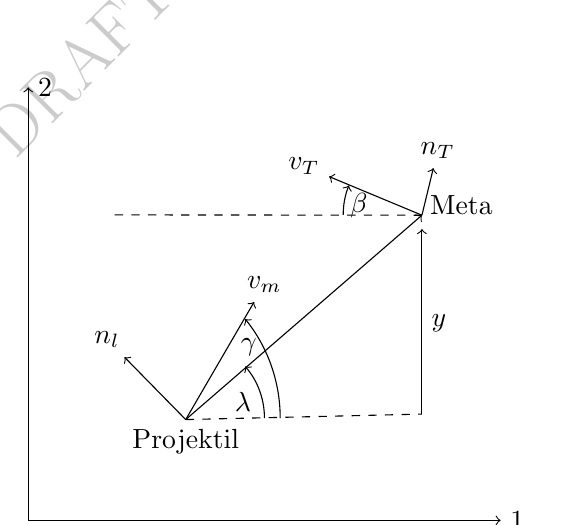
\begin{tikzpicture}
        \draw [->](0,0)--(0,5.5) node[right]{$2$};
        \draw [->](0,0)--(6,0) node[right]{$1$};
        \node[] at (2,1) (m){Projektil};
        \node[] at (5,4) (t){};
        \node[right of = t, node distance =0.5cm] (){Meta};
        \draw[->] (m.north) -- (t.south);
        \node[]at(3,3)(vm){$v_m$};
        \draw[->](m.north)--(vm);
        \node[] at (1,2.3) (nl){$n_l$};
        \draw[->] (m.north)--(nl);
        \draw[dashed] (m.north) -- (5,1.35);
        \node[anchor = west] at (2.5, 1.5) () {$\lambda$};
        \draw[->] (3,1.3) arc (0:41:1);
       \draw[->](3.2,1.3) arc (0:39:2);
       \node[] at (2.8, 2.2) () {$\gamma$};
       \draw[dashed] (t.south) -- (1,3.88);
       \node[] at (3.5,4.5)(vt){$v_T$};
       \draw[->] (t.south) -- (vt);
       \node[] at (5.2, 4.7) (nt){$n_T$};
       \draw[->](t.south) -- (nt);
       \draw[->] (5,1.35)--(5,3.7);
       \node[anchor = west] at (5, 2.5) (){$y$};
       \draw[->] (4, 3.88) arc (180:158:1);
       \node[] at (4.2,4) (){$\beta$};
\end{tikzpicture}   
    \caption{Linearizacija jednačina proporcionalne navigacije}
    \label{fig:linear}
\end{figure}
\noindent Linearizacija se može lahko izvršiti ako se definišu nove veličine koje su prikazane na slici \ref{fig:linear}.
Relativno ubrzanje se može odrediti sa slike i iznosi:
\begin{equation}
    \ddot{y}=n_T\cos\beta-n_c\cos\lambda
\end{equation}
Ako su uglovi leta mali, tada vrijedi:
\begin{equation}
    \ddot{y}=n_T-n_c
\end{equation}
Slično tako vrijedi:
\begin{equation}
    \lambda = \frac{y}{r}
\end{equation}
Za čeoni slučaj vrijedi:
\begin{equation}
    v_{cl}=v_M+v_t
\end{equation}
Za potjeru vrijedi:
\begin{equation}
    v_{cl}=v_M-v_t
\end{equation}
Sada se može linearizirati i jednačina za udaljenost:
\begin{equation}
    r(t)=v_{cl}(t_F-t)
\end{equation}
gdje je $t_F$ ukupno vrijeme leta.\\
Definišimo i veličinu \textit{time to go} $t_{go}$:
\begin{equation}
    t_{go}=t_F-t
\end{equation}
Linearizirani promašaj se definisše kao udaljenost mete i projektila na kraju leta, ili:
\begin{equation}
    Miss=y(t_f)
\end{equation}
\section{Petlja navođenja i zero effort miss}
Ranije je pokazano da vrijedi:
\begin{equation}
    \dot{\lambda}(t)=\frac{\dot{y}(t)r(t)+y(t)v_{cl}}{r^2}
\end{equation}
Kako vrijedi $r=v_{cl}t_{go}$, tada se dobija:
\begin{equation}
    \dot{\lambda}(t)=\frac{\dot{y}(t)t_{go}+y(t)}{v_{cl}t_{go}^2}
\end{equation}
Definišimo sada veličinu \textit{Zero effort miss}, koja predstavlja buduće relativno rastojanje projektila i mete:
\begin{equation}
    ZEM=\dot{y}(t)t_{go}+y(t)
\end{equation}
pa se dobija:
\begin{equation}
    \dot{\lambda}(t)=\frac{ZEM}{v_{cl}t_{go}^2}
\end{equation}
Ako se pretpstavi da će se pod uticajem ubrzanja $a_c$ postići sudar, $ZEM$ se može smatrati 
budućom tačkom susreta, pa se zakon vođenja proprcionalne navigacije može iskazati kao:
\begin{equation}
    a_c(t)=N\frac{ZEM}{t_{go}^2}
\end{equation}
Sada se vidi da je normalno ubrzanje projektila direktno proprorcionalnu $ZEM$-u i inverzno proporcionalno
kvadratu preostalom vremenu leta, što znači da se generiše veće ubrzanje što je susret bliži.
Pošto se $ZEM$ posmatra kao buduća tačka susreta, koja se računa na osnovu znanja ili pretpostavki 
budučeg kretanja mete, PN vođenje se smatra prediktivnim. $ZEM$ je koristan jer se može izračunati 
mnoštvom metoda uključujući i on-line numeričku integraciju nelinearnih diferencijalnih jednačina projektila 
i mete. Pretohdno izvedene linaerizovane jednačine proporcionalne navigacije se mogu 
prikazati blok dijagramom kao na slici \ref{fig:homing}.
\begin{figure}[htp]
    \centering
    \begin{tikzpicture}[auto, node distance=2cm]
        \node[input, name = nt] (nt){$n_T$};
        \node[sum, right of = nt, node distance=1cm](sum){};
        \node[block, right of = sum] (int2){$\frac{1}{s^2}$};
        \node[block, right of = int2] (div) {$\frac{1}{v_{cl}(t_f-t)}$};
        \node[block, right of=div](seeker){$s$};
        \node[block, below of = div](law){$Nv_{cl}$};
        \node[block, left of = law](dyn){$\frac{1}{1+T_ms}$};
        \node [output, right of=seeker, node distance=1cm] (output) {};
        \node (a) at ($(int2)!0.5!(div)$){};
        \node (miss) at ($(a) -(0, 0.145cm) $){};
        \node[above of = miss, node distance=1.5cm] (missArr){Promašaj};
        \draw[->] (miss)--(missArr);
        \node at (nt) [anchor = south ](){$n_T$};
        \node[left of = dyn, node distance = 1cm, anchor = south] () {$n_L$};
        \node[anchor = south] () at ($(dyn)!0.5!(law)$) {$n_C$};
        \node[right of = seeker,anchor = south, node distance = 1 cm] () {$\dot{\lambda}$}; 
        \draw[->](nt)--node[pos=0.95] {$+$}(sum);
        \draw[->](sum)--(int2);
        \draw[->](int2)--(div);
        \draw[->](div)--(seeker);
        \draw[->](output)|-(law);
        \draw[->](law)--(dyn);
        \draw [-] (seeker) -- node [name=y] {}(output);
        
        \draw[->](dyn)-|node[pos=0.99] {$-$}(sum);
        
        \end{tikzpicture}
    \caption{Petlja navođenja}
    \label{fig:homing}
\end{figure}
Ulaz sistema je ubrzanje mete, a u 
povratnoj sprezi se nalazi upralvjački zakon. Pretpostavlja se da je model trekera idealni diferencijator i sistem 
za navođenje ne uvodi nikakvo kašnjenje. U stvarnosti, sistem za navođenje se modelira prenosnom 
funkcijom prvog reda, tj:
\begin{equation}
    \frac{n_L}{n_c}=\frac{1}{1+sT}
\end{equation}
,gdje je $n_L$ ostvareno ubrzanje projektila, a $n_c$ zahtjevano ubrzanje projektila.
\begin{figure}[!ht]
    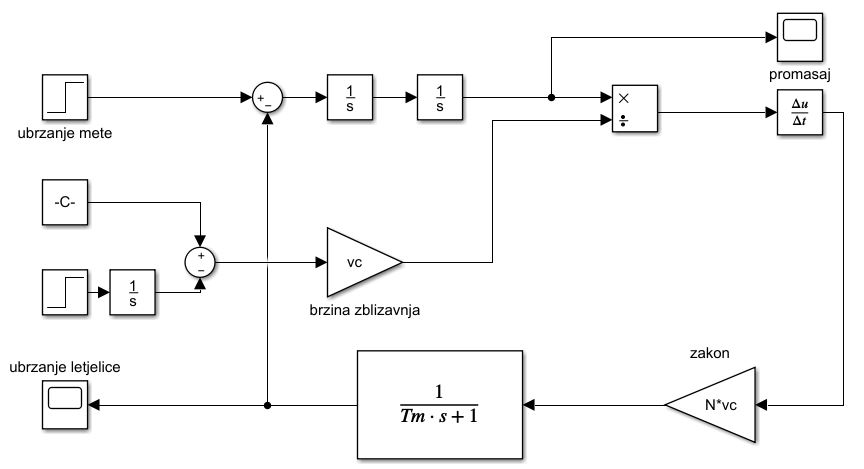
\includegraphics[scale = 0.6]{homingSimulink.JPG}
    \caption{Proporcionalana navigacija u Simulinku}
    \label{fig:simProp}
\end{figure}
Koristeći Simulink dijagram sa slike \ref{fig:simProp} izvršene su simulacije za $N=4$ i $N=5$
pri ubrzanju mete od $3g$. Ubrzanja projektila su prikazana na grafu \ref{fig:propAcc}.
\begin{figure}[htp!]
    \centering
    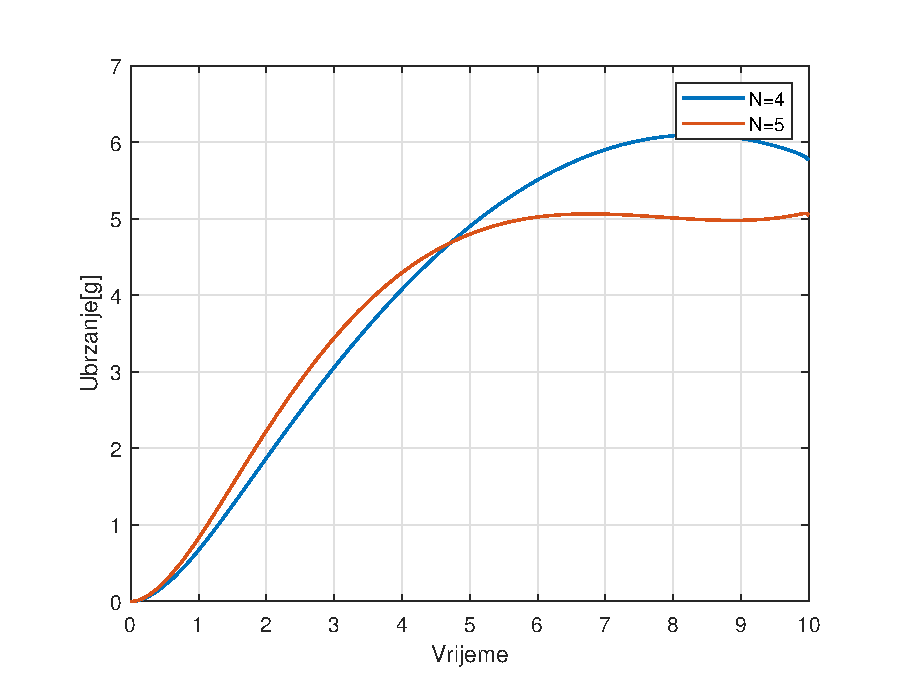
\includegraphics[scale = 0.5]{propAccPlot.eps}
    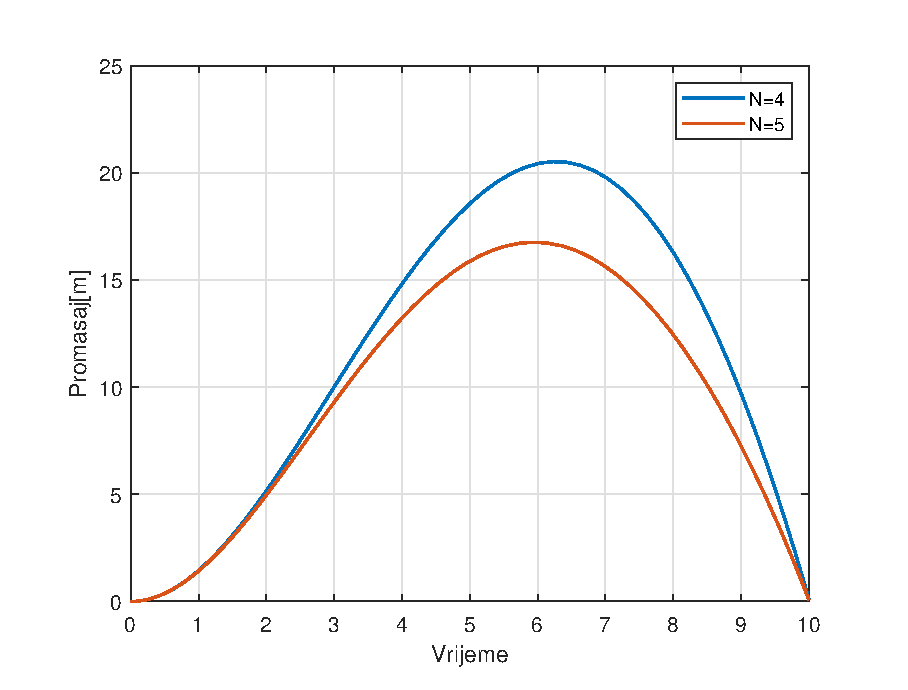
\includegraphics[scale = 0.5]{missProp.eps}
    \caption{Ubrzanja projektila i promašaj za $N=4$ i $N=5$}
    \label{fig:propAcc}
\end{figure}
Vidi se da veći efektivni navigacijski odnos zahtjeva manje ubrzanje projektila pa su time 
smanjeni i zahtjevi za performanasam projektila, međutim veći efektivni navigacijski odnos 
daje manji promašaj što se vidi na grafiku za promašaj na slici \ref{fig:propAcc}. 
U oba slučaja ostvaren je sudar unutar deset sekundi. U nastavku je na slici \ref{fig:simAugProp} prikazan 
simulink model izmjenjene proporcionalne navigacije.
\begin{figure}[!ht]
    \centering
    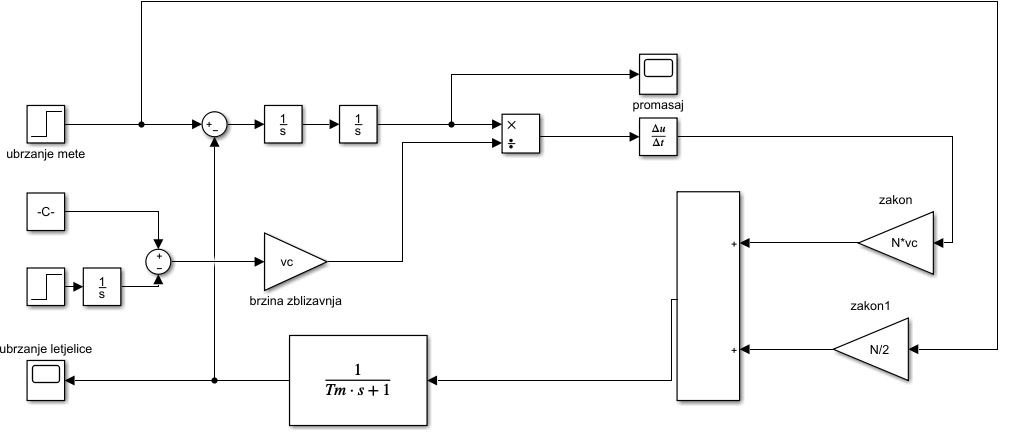
\includegraphics[scale = 0.6]{augPropSim.JPG}
    \caption{Simulink model izmjenjene proporcionalne navigacije}
    \label{fig:simAugProp}
\end{figure}
Ubrzanje projektila i promašaj su prikazana na graficima na slici \ref{fig:augPropGraf}.
\begin{figure}[!ht]
    \centering
    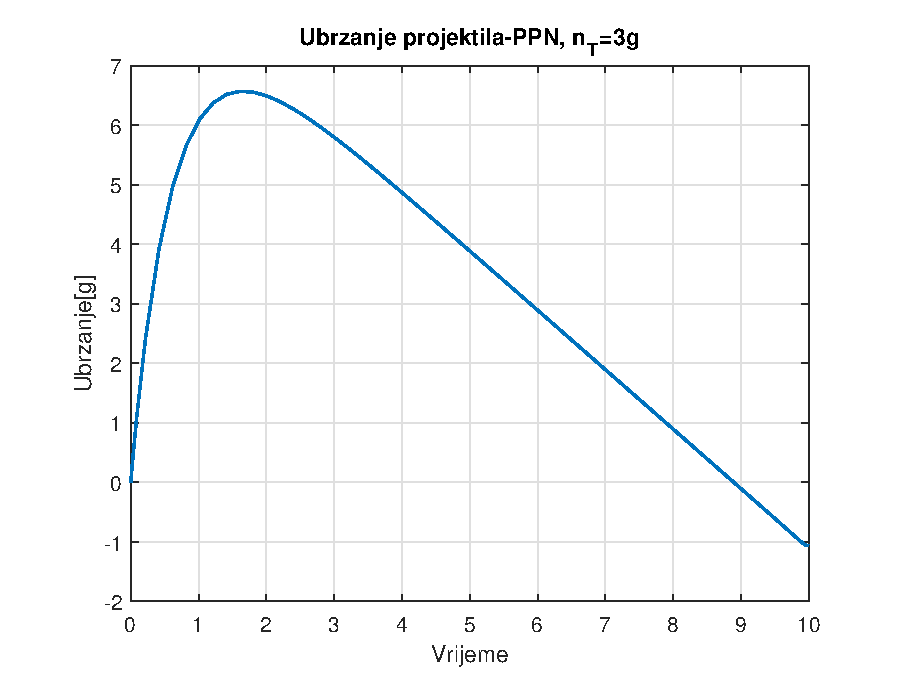
\includegraphics[scale = 0.5]{augPropAcc.eps}
    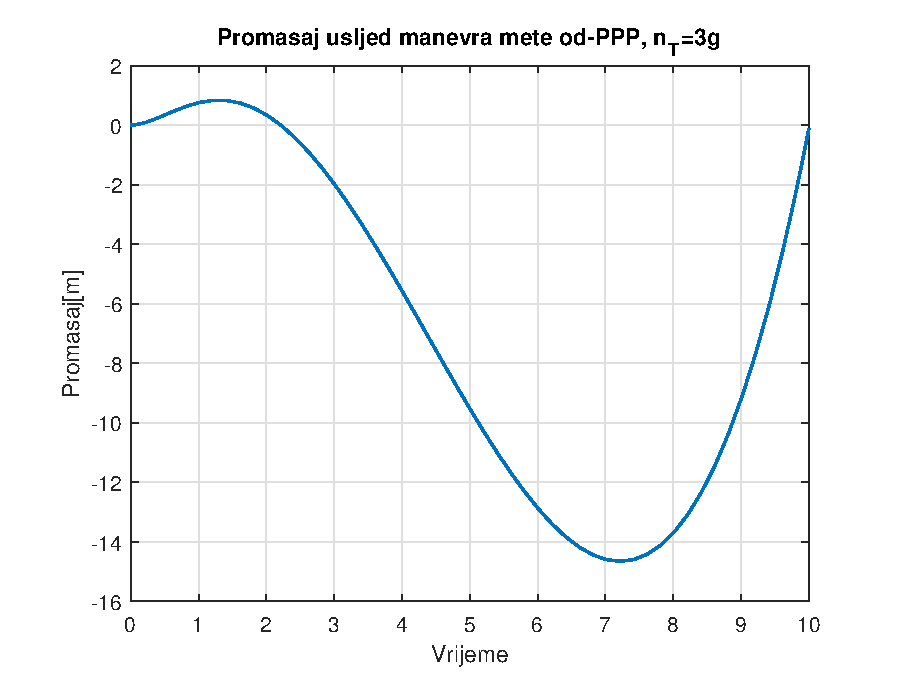
\includegraphics[scale = 0.5]{augPropMiss.eps}
    \caption{Ubrzanje projektila i promašaj vođen promjenjenom proporcionalnom naivgacijom, $N=3$}
    \label{fig:augPropGraf}
\end{figure}
Sada se konačno vidi da i kod proporcionalne navigacije i kod promjenjene proporcionalne navigacije 
se grantuje sudar unutar vrmena leta ako se izabere $N=3$. Dalje se vidi da 
ubrzanje projektila kod promjenjene proporcionalne navigacije počinje od nula za razliku od čiste proporcionalne 
navigacije. Kod promjenjene proporcionalne navigacije promašaj može postati negativan što iziskuje 
promjenu smjera normalnog ubrzanja projektila. 
\section{Adjungovani sistem i petlja navođenja}
Direktna simulacija lineariziranih jednačina proporcionalne navigacije se uvijek može
koristiti za generisanje upravljačkog signala(tj. normalnog ubrzanja) projektila
ali je tehnika nazvana \textit{adjungovana tehnika} historijski bila glavni računarski 
alat za dizajn i analizu vođenih projektila. Adjungovana tehnika je zasnovana 
na impulsnom odzivu sistema i koristi se  za analizu LTI sistema kao što je 
petlja navođenja projektila. Koristeći ovu tehniku mogu se dobiti tačne vrijednosti 
bilo koje veličine u datom trenutku.\\
Poznato je da je odziv sistema na prooizvoljni ulaz potpuno određen impulsnim odzivom sistema, pa 
tj. vrijedi da je odziv linearnog sistema dat sa:
\begin{equation}
    y(t)=\int_o^tu(\tau)h(t,\tau)d\tau
\end{equation}
Fizikalno, impuslni odziv $h(t-\tau)$ predstavlja odziv sistema na impulsnu pobudu koja 
se primjeni na sistem u trenutku $\tau$. Prema tome određivanje odziva sistema zahtjeva analitičku 
formu impulsnog odziva. Svaki linearni sistem ima i svoj adjungovani sistem i veza između impulsnog 
odziva linearnog sistema i njegovog adjungovanog sistema je data sa:
\begin{equation}
    h^*(t_f-\tau,t_f-t)=h(t,\tau)
\end{equation}
Ako se uzme da je ulaz sistema Heavysideov impuls, tada je odziv sistema dat sa:
\begin{equation}
    y(t)=a\int_0^t h^*(t_f-\tau,t_f-t)d\tau
\end{equation}
,nakon uvođenja smjene $x=t_f-\tau$, dobija se:
\begin{equation}
    y(t)=a\int_{t_f-t}^{t_f}h^*(x,t_f-t)dx
\end{equation}
Pošto je veličina od interesa promašaj na kraju leta uzima se $t_f=t$, pa prethodna relacija
postaje:
\begin{equation}
    y(t_f)=a\int_{0}^{t_f}h^*(x,0)dx
\end{equation}
Vidi se da se integracija vrši po posmatranom vremenu i da ne zavisi od trenutka primjene impulsa na adjunogvani sistem. 
Ovo znači da se izlaz u trenutku $t_f$ može dobiti primjenjujući impuls u početnom trenutku, te zatim integrišući ulaz. 
Konstrukcija adjungovanog modela se vrši prema naredna tri koraka:
\begin{enumerate}
    \item Pretvoriti sve ulaze sistema u impulse
    \item Zamjeniti $t$ sa $t_f-t$ i obratno na mjestima gdje se vrijeme pojavljuje kao argument
    \item Promjeniti smjer toka svih signala, mjenjajući sume sa čvorovima i obratno
\end{enumerate}
Koristeći navedena pravila dobija se adjungovana petlja navođenja prikazana na slici \ref{fig:adjHoming}, s tim 
da je kao smetnja u sistem dodata još i početna greška nišanjenja data sa $v_Me_q$ ,za $v_M=610\frac{m}{s}$ i $e_q=20\deg$.
Sada je moguće dobiti promašaj usljed manevra mete i promašaj usljed početne greške nišanjenja sve u jednoj 
simulaciji!
\begin{figure}[!ht]
    \centering
    \begin{tikzpicture}[auto, node distance=2cm,>=latex']
        \node[block] (nt) {$n_T$};
        \node[block, right of = nt](int1){$\frac{1}{s}$};
        \node[right of = int1] (center){};
        \node[block, right of = center](int2){$\frac{1}{s^2}$};
        \node[sum, right of = int2, node distance = 2cm](sum){+};
        \node[block, right of = sum](div){$\frac{1}{v_{cl}t}$};
        \node[block, below of = int2](law){$-\frac{N'v_{cl}s}{1+sT_m}$};
        \node[name = delta, above of = sum, node distance = 1.5cm](delta){$\delta(0)$};
        \node[left of = nt](out){Promašaj};
        \node[below of = out, node distance=0.3cm](out2){usljed};
        \node[below of = out2, node distance=0.3cm](){manevra mete};
        \node[right of = div](a){};
        \node at (center) [anchor = south west]{$\dot{x}_1$};
        \node[block, above of = center,node distance = 1.5cm](head){$-v_Me_q$};
        \node[above of = head, node distance = 1.5cm](m){};
        \node[right of = m, node distance =1cm](q){Promašaj};
        \node[below of = q, node distance = 0.3cm](w){usljed};
        \node[below of = w, node distance = 0.3cm](e){greške};
        \node[right of =e , node distance = 1.5cm](){nišanjenja};
        \draw[->](head)--(m);
        \draw[->](center.south)-- ++(0,0.1)--(head);
        \draw[->](delta)--(sum);
        \draw[->](sum)--(int2);
        \draw[->](int1)--(nt);
        \draw[->](div)--(sum);
        \draw[->](int2)--(int1);
        \draw[->](center.south)-- ++(0,0.13)|-(law);
        \draw[-](law)-|(a.east) -- ++(0,0.0215);
        \draw[->](a.east)-- ++(0.0215,0)--(div);
        \draw[->](nt)--(out);
        \end{tikzpicture}
    \caption{Adjungovana petlja navođenja}
    \label{fig:adjHoming}
\end{figure}
Jedinični impuls se može predstaviti kao početni uslov kod prvog integratora. Na slici \ref{fig:simAdj} 
je predstavljen Simulink dijagram adjungovanog sistema.
\begin{figure}[!ht]
    \centering
    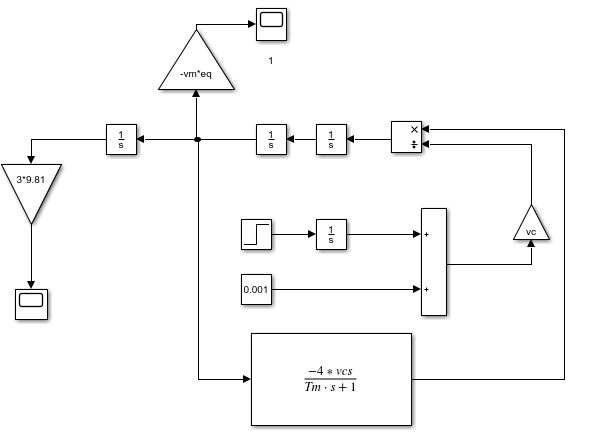
\includegraphics[scale= 0.7]{simAdj.JPG}
    \caption{Simulink dijagram adjungovanog sistema}
    \label{fig:simAdj}
\end{figure}
Simulacija za date vrijednosti daje promašaj usljed početne greške nišanjenja i 
promašaj usljed konstantnog manevra mete i oni su prikazani na slici \ref{fig:adjDet}.
\begin{figure}[!ht]
    \centering
    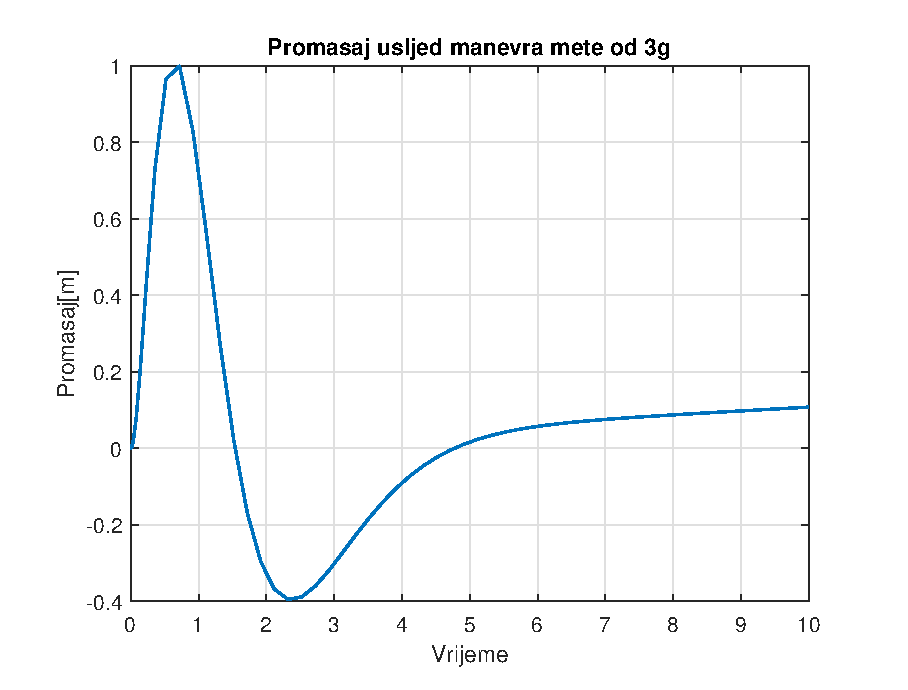
\includegraphics[scale=0.5]{missAdjDet.eps}
    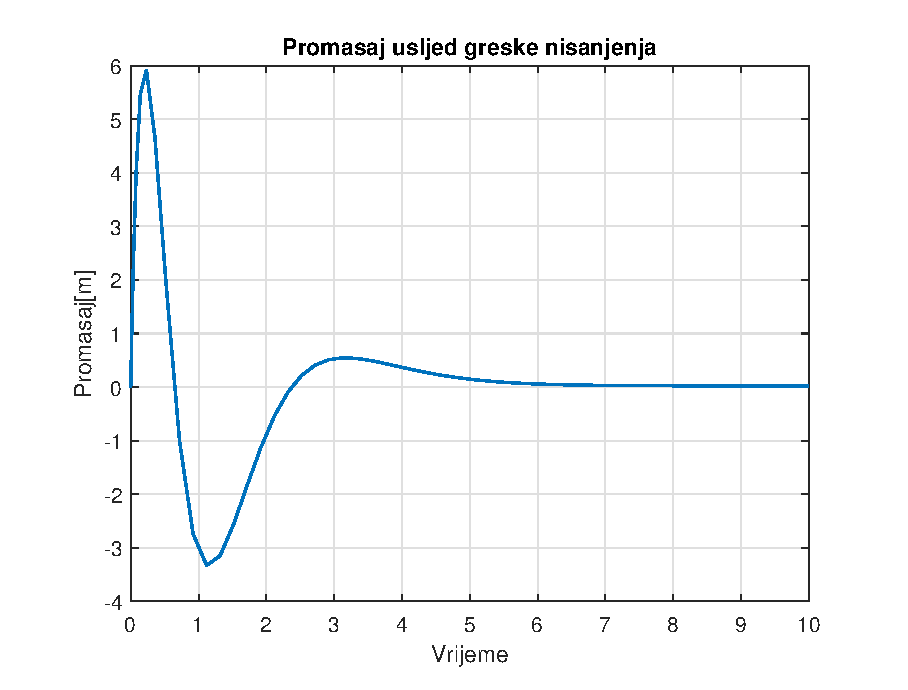
\includegraphics[scale=0.5]{missHead.eps}
    \caption{Odzivi adjungovanog sistema}
    \label{fig:adjDet}
\end{figure}
\section{Adjungovani stohastički sistemi}
Pored mnoštva informacija koje adjungovani sistem daje pri analizi determinističkih 
sistema, adjugnovana tehnika je dosta korisna pri analizi stohastičkih sistema što je 
naročito korisno pri analizi petlje navođenja jer su manevri mete u stvarnosti stohastički. 
Prije nego se prikaže upotreba adjungovane tehnike na petlji navođenja sa stohastičkim 
ulazima, potrebno je se prisjetiti nekoliko važnih definicija.\\
Očekivana vrijednost slučajne promjenljive $x$ čija funkcija gustoće vjerovatnoće $p(x)$ je definisana sa:
\begin{equation}
    E(x)=\int_{-\infty}^{\infty}xp(x)dx
\end{equation}
Standardna devijacija je data sa:
\begin{equation}
    \sigma = \sqrt{E(x^2)-E^2(x)}
\end{equation}
Autokorelaciona funkcija je data sa>
\begin{equation}
    \phi_{xx}(t_1,t_2)=E[x(t_1)x(t_2)]
\end{equation}
Autokorelaciona funkcija predstavlja sličnost dvaju identičnih funkcija 
pri čemu su one smaknute za neki vremenski interval.
Fourieova transformacija autokorelacione funkcije se zove \textit{spektralna 
gustoća snage} i data je sa:
\begin{equation}
    \Phi_{xx}=\int_{-\infty}^{\infty}\phi_{xx}(\tau)e^{-j\omega\tau}d\tau
\end{equation}
Kod bijelog šuma spektralna gustoća snage je konstanta tj.
\begin{equation}
    \Phi_{xx}=\phi_{0}
\end{equation}
Autokorelaciona funkcija bijelog šuma je delta impuls tj. 
\begin{equation}
    \phi_{xx}=\Phi_{0}\delta(t)
\end{equation}
Ovo znači da je bijeli šum samo u jednoj tački identičan samom sebi. 
Kod stohastičkih sistema, izlaz je opisan očekivanom vrijednosšću kvadrata izlaza. 
Prema tome, ako su ulazi tipa bijelog šuma tada vrijedi:
\begin{equation}
    y^2(t)=\int_{-\infty}^tx(\tau_1)h(t,\tau_1)d\tau_1\int_{-\infty}^tx(\tau_2)h(t,\tau_2)d\tau_2
\end{equation}
Ako je $x(t)$ slučajna promjenljiva, može se naći i očekvana vrijednost kvadrata izlaza:
\begin{equation}
    E[y^2(t)]=\int_{-\infty}^t\int_{-\infty}^th(t,\tau_1)h(t,\tau_2)E[x(\tau_1)x(\tau_2)]d\tau_1d\tau_2
\end{equation}
Ako je ulaz $x(t)$ tipa bijelog šuma spektralne gustoće snage $\Phi$, tada se prethodni 
dovjni integral može pojednostaviti zbog impuslne prirode autokorelacione funkcije 
bijelog šuma, pa vrijedi:
\begin{equation}
    E[y^2(t)]=\Phi \int_{-\infty}^t h^2(t,\tau)d\tau
\end{equation}
Sada se prisjetimo da je impulsni odziv adjungovanog sistema $h^*(t_f-\tau,t_f-t)=h(t,\tau)$
 i nakon uvođenja smjene $x=t_f-\tau$, dobija se:
\begin{equation}
    E[y^2(t)]=\Phi\int_{t_f-t}^{t_f}[h^*(x,t_f-t)]^2dx
\end{equation}
Pošto je u interesu promašaj na kraju leta, to je:
\begin{equation}
    E[y^2(t_f)]=\Phi\int_{0}^{t_f}[h^*(x,0)]^2dx
\end{equation}
Sada se vidi da se očekivana vrijednost kvadrata izlaza može dobiti tako što se 
kvadrira i integrira izlaz stohstičkog sistema i to sve u toku samo jedne simulacije. 
Prednost adjungovane metode postaje veća kada se uzme u obzir da na stohastički sistem 
može djelovati više slučajnih ulaza. Kod adjungovane metode, ulazi postaju izlazi pa se 
superpozicijom pri samo jednoj simulaciji može dobiti tačna statisička analiza stohastičkog sistema i 
analiza utjecaja svakog ulaza(tipa bijelog šuma) na performanse sistema. \\
Sada pretpostavimo da meta izvodi manevar konstantnog normalnog ubrazanja i da ga 
počinje izvoditi u trenutku $T$ koji je dat uniformnom raspodjelom i to tako da vrijedi:
\begin{equation}
    p(t)=
    \begin{cases}
        \frac{1}{t_f}, \quad za 0\leq t\leq t_f\\
        0 \qquad za t\geq T\\
    \end{cases}
\end{equation}
Prema tome ulaz u petlju vođenja je dat sa:
\begin{equation}
    x(t)=n_Tu(t-T)
\end{equation}
Ovo znači da je vjerovatnoća pojave manevra jednako vjerovatno u toku cijelog leta. 
Prema tome, autokorelaciona funkcija ulaza u petlju vođenja je:
\begin{equation}
    \phi_{xx}(t_1,t_2)=\int_{-\infty}^{\infty}x(t_1)x(t_1)p(T)dT
\end{equation}
pa se dobija:
\begin{equation}
    \phi_{xx}(t_1,t_2)=\int_{0}^{t_f}n_T(t_1-T)n_T(t_2-T)\frac{dT}{t_f}
\end{equation}
Ako se pretpostavi da je $0<t_1<t_2<t_f$, dobija se autokorelacione funkcija ulaza:
\begin{equation}
    \phi_{xx}(t_1,t_2)=\frac{n_T^2}{t_f}\int_{0}{t_1}dT
    \label{eq:autoCorrxx}
\end{equation}
Autokorelaciona funkcija sistema sa impulsnim odzivom $h(t)$ koji je vođen bijelim 
šumom se može izraziti kao:
\begin{equation}
    \phi_yy(t_1,t_2)=\int_{-\infty}^{t_1}h(t_1-\tau)\int_{-\infty}^{t_2}h(t_2-\tau)\phi_{uu}(\tau_1,\tau_2)d\tau_1d\tau_2
\end{equation}
Gdje je $\phi_{uu}(t_1,t_2)= \Phi_u\delta(\tau_1-\tau_2)$, autokorealciona funkcija bijelog šuma
i $\Phi_u$ je spektralna gustoće snage i pretpostavlja se da je ona konstantna za cijelo vrijeme leta tj. da vrijedi:
\begin{equation}
    \Phi_u(t) = \begin{cases}
        \Phi_u, \quad 0 \leq t \leq t_f \\
        0, \quad \text{inače} 
    \end{cases}
\end{equation}
Pa se dobija:
\begin{equation}
    \phi_yy(t_1,t_2) = \Phi_u\int_0^{t_1}h(t_1-\tau)h(t_2-\tau)d\tau1
\end{equation}
Sada poredeći prethodnu jednačinu sa \ref{eq:autoCorrxx} zaključuje se da 
su dvije autokorelacione funkcije iste ako je: 
\begin{eqnarray}
    \Phi_u =\frac{n_T^2}{t_f} \\
    h(t)=1
\end{eqnarray}
Sada se vidi da je manevar konstante amplitude $n_T$, kod koga je vrijeme 
početka djelovanja uniformno raspoređeno u toku vremena leta $t_f$ ima istu 
autokorelacionu funkciju kao i linearni sistem sa prenosnom funkcijom $H(s)=\frac{1}{s}$ 
na koji djeluje bijeli šum spektralne gustoće snage dat sa: 
\begin{equation*}
    \Phi_u(t) = \begin{cases}
        \Phi_u, \quad 0 \leq t \leq t_f \\
        0, \quad \text{inače}
    \end{cases}
\end{equation*}
Sada će se prikazati primjena adjungovane tehnike na sthastički sistem. Važe ista pravila 
za kreiranje adjungovanog sitema kao i ranije sa jednim dodatnim pravilom da se 
svi stohastički ulazi se moraju modelirati kao bijeli šum koji na kraju postaju 
izlazi adjungovanog sistema. Pošto se ulaz originalnog sistema modelira kao bjeli šum 
kroz integrato, adjungovani model će promjeniti tok signala i kvadrirati i integrisati izlaz.
Dobijeni adjungovani model je prikazan na slici \ref{fig:adjStohastic}.
\begin{figure}[!ht]
    \centering

    \begin{tikzpicture}[auto, node distance=2cm,>=latex']
        \node[block] (nt) {$\frac{1}{s}$};
        \node[block, right of = nt](int1){$\frac{1}{s}$};
        \node[right of = int1] (center){};
        \node[block, right of = center](int2){$\frac{1}{s^2}$};
        \node[sum, right of = int2, node distance = 2cm](sum){+};
        \node[block, right of = sum](div){$\frac{1}{v_{cl}t}$};
        \node[block, below of = int2](law){$-\frac{N'v_{cl}s}{1+sT_m}$};
        \node[name = delta, above of = sum, node distance = 1.5cm](delta){$\delta(0)$};
        \node[left of = nt](out){};
        \node[right of = div](a){};
        \node[left of = nt, node distance = 1.5cm](b){};
       \node[block, below of = b, node distance = 1cm](sq){$()^2$};
       \node[block,below of = sq, node distance = 1.5cm](ro){$\frac{1}{s}$};
       \node[block,right of = ro](gain){$\frac{n_T^2}{t}$};
       \node[right of = gain](out1){$E\left[y^2(t_f)\right]$};
       \draw[->](gain)--(out1);
       \draw[->](ro)--(gain);
       \draw[->](sq)--(ro);
       \draw[->](nt)-|(sq);
        \draw[->](delta)--(sum);
        \draw[->](sum)--(int2);
        \draw[->](int1)--(nt);
        \draw[->](div)--(sum);
        \draw[->](int2)--(int1);
        \draw[->](center.south)-- ++(0,0.13)|-(law);
        \draw[-](law)-|(a.east) -- ++(0,0.0215);
        \draw[->](a.east)-- ++(0.0215,0)--(div);
        \end{tikzpicture}
    \caption{Adjungovani stohastički model}
    \label{fig:adjStohastic}
\end{figure}
Na slici \ref{fig:adjStohasticSimm} je prikazan Simulink model ajdungovanog stohastičkog sistema. 
Impulsni signal je u Simulink modelu unešen kao početni uslov na odgovarajućem integratoru. 
\begin{figure}[!ht]
    \centering
    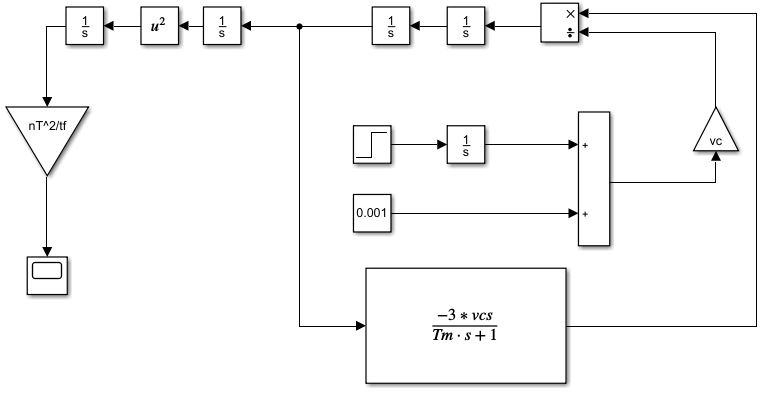
\includegraphics[scale=0.5]{adjStohastic.JPG}
    \caption{Simulink model ajdungovanog stohastičkog sistema}
    \label{fig:adjStohasticSimm}
\end{figure}
Dobija se očekivana vrijednost kvadrata promašaja kao što je prikazano na grafiku \ref{fig:stohGraf}
\begin{figure}[!ht]
    \centering
    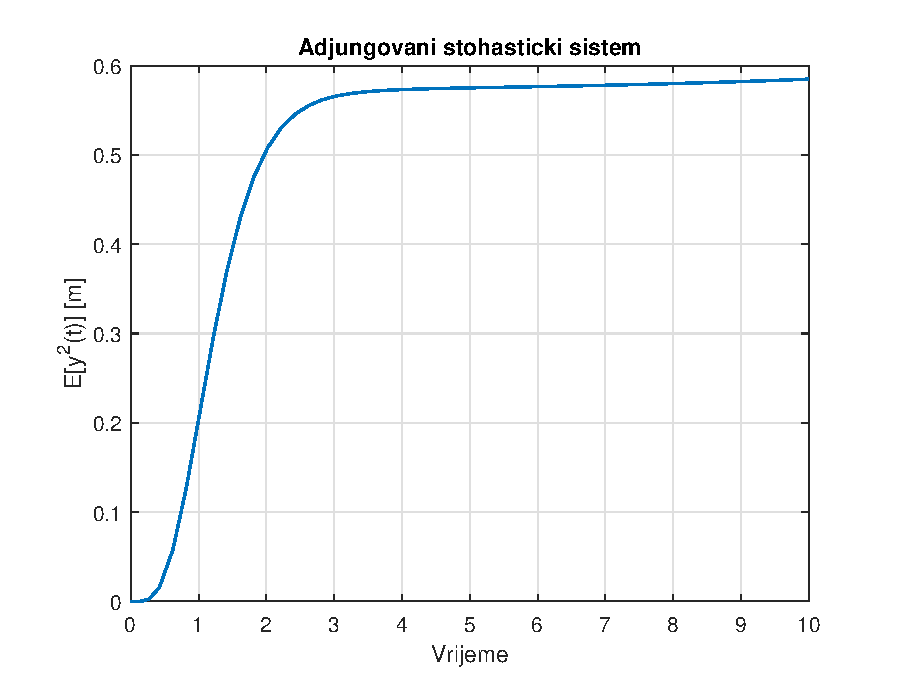
\includegraphics[scale=0.5]{adjStohasticSim.eps}
    \caption{Očekivana vrijednost kvadrata promašaja}
    \label{fig:stohGraf}
\end{figure}
Vidi se da je očekivana vrijednost kvadrata promašaja naglo porasla u prve tri sekunde leta. 
Ovo je zbog toga što je upravo u tom intervalu promašaj najveći, nakon toga promašaj počinje opadati.




%\printbibliography

\end{document}